\documentclass[10pt]{article}
\usepackage{amscd,amsfonts,amssymb,amstext,latexsym} 
\usepackage{amsmath,mathbbol,mathrsfs,stmaryrd, mathtools} 

\usepackage {algorithm} 
\usepackage{theoremref}
\usepackage[T1]{fontenc}
\usepackage[english]{babel} 
\usepackage {enumerate}
\usepackage{url}
\usepackage[noend]{algpseudocode}
\usepackage{float}
\usepackage{graphics} 
\usepackage{tikz}
\usepackage[width=14.8cm,left=3cm,margin=1in]{geometry}
\usetikzlibrary{automata,calc}
%\usepackage{tgtermes} 
\usepackage{listings}
\usepackage{mathptmx}
\usepackage{fancyhdr}
\usepackage{verbatim}
\usepackage{enumitem}
\usepackage{booktabs}
\usepackage[flushleft]{threeparttable}
\usepackage{listings}
\usepackage{verbatim}
\usepackage{fancyhdr}
\usepackage{multirow,multicol}
\usepackage{color}
\usepackage[toc,page]{appendix}
\usepackage{changepage}

\usepackage[utf8]{inputenc}
\usepackage{graphicx}


\usepackage[colorlinks=true,linkcolor=blue,citecolor=blue,urlcolor=blue]{hyperref}
\usepackage{tabto}
\lstset{ %
language=C,                % choose the language of the code
basicstyle={\ttfamily},       % the size of the fonts that are used for the code
backgroundcolor=\color{white},  % choose the background color. You must add \usepackage{color}
showspaces=false,               % show spaces adding particular underscores
aboveskip=6mm, 
%belowskip=3mm, 
numbers=left, numberfirstline=false, numberblanklines=false,
numberstyle=\tiny\color{gray}, numbersep= 5pt, 
showstringspaces=false,         % underline spaces within strings
showtabs=false,                 % show tabs within strings adding particular underscores
%frame=single,           % adds a frame around the code
%frame = tb, 
frame = none, 
tabsize=2,          % sets default tabsize to 2 spaces
captionpos=b,           % sets the caption-position to bottom
breaklines=true,        % sets automatic line breaking
breakatwhitespace=false,    % sets if automatic breaks should only happen at whitespace
escapeinside={\%*}{*)}          % if you want to add a comment within your code
}
%\graphicspath{{../../pics/}}
\fancypagestyle{plain}{
\fancyhf{}
\rhead{School of Computer Science and Applied Mathematics\\ 
%\noindent\rule{15.4cm}{0.4pt}\\
\footnotesize{\textsc{University of the Witwatersrand, Johannesburg}}}
\lhead{
\includegraphics[scale=0.08]{witslogo_h.png}}
\fancyfoot[C]{\thepage}
\renewcommand{\headrulewidth}{0.4pt}
}

%\textwidth=16.8cm 
%\textheight=22.6cm 
\evensidemargin 0pt 
\oddsidemargin 0pt 
\leftmargin 0pt 
\rightmargin 0pt 
\setlength{\topmargin}{0pt} 
\setlength{\footskip}{50pt}
\setlength{\parindent}{0pt}
\setlength{\parskip}{0.5em}
\linespread{1} 
% 
\makeatletter
\newcommand{\rmnum}[1]{\romannumeral #1}
\newcommand{\Rmnum}[1]{\expandafter\@slowromancap\romannumeral #1@}
\makeatother

%Custom commands for logical operators and other pseudocode stuff
\algnewcommand\AND{\textbf{ and }}
\algnewcommand\OR{\textbf{ or }}
\algnewcommand\NOT{\textbf{not}}
\algnewcommand\BREAK{\textbf{break}}
\algnewcommand\RETURN{\textbf{return }}

\begin{document}
\title{COMS4040A Assignment 2 -- Report}
\author{Tamlin Love (1438243) - BSc Hons}
\date{\today} 
\maketitle 
%\thispagestyle{empty}
\pagestyle{fancy}
\fancyhf{}
\fancyhead[R]{\thepage}
\fancyhead[L]{COMS4040A Assignment 2}
%\vskip 3mm 
%\pagenumbering{roman}
%\newpage
\pagenumbering{arabic} 
\vspace{-1.5cm}
\section{Introduction}\label{Introduction}
Discrete Image Convolution is a widely used technique in digital image and signal processing. It can achieve a huge variety of effects, from blurring and sharpening to edge detection and noise removal. 
\\
Consider a discrete image $I \in \mathbb{R}^{M \times N}$ where each $Y(i,j) \in [0,1]$. Consider also a discrete filter $F \in \mathbb{R}^{L \times P}$. Then the discrete convolution of $I$ by $F$ is defined as:
\begin{equation}
(I*F)(i,j) = \sum_{s=0}^{L-1}\sum_{t=0}^{P-1} I(i-s,j-t)F(s,t),
\end{equation}
where $i\in[0,M-1]$ and $j\in[0,N-1]$.
\\
In serial, this can be an expensive operation as it has an asymptotic time complexity of $\mathcal{O}(MNLP)$. However, because the calculation of each pixel $I(i,j)$ depends only on its local neighbourhood, we can parallelise the problem to improve efficiency. In this report, we consider several approaches to parallelising the problem on a GPU using CUDA. Before we can discuss these approaches, however, we must first discuss the different types of memory on a GPU.
\subsection{GPU Memory}
On the GPU there are 5 types of memory \cite{wang19}:
\begin{itemize}
\item \textbf{Local Memory} - each thread has its own local memory which is not shared with any other threads, thus limiting its use to temporary variables in the convolution calculation.
\item \textbf{Shared Memory} - this type of memory is shared among threads in a block. It is typically very fast, but is also quite small (48 KB on a Nvidia GTX 1060\cite{nvidia19})
\item \textbf{Global Memory} - global memory resides on the device and is accessible by all grids. As a consequence, it is fairly slow.
\item \textbf{Constant Memory} - constant memory is a fast read-only memory type that is accessible by all grids. It is optimised for being read by multiple threads, but is fairly small (64 KB on a Nvidia GTX 1060\cite{nvidia19}).
\item \textbf{Texture Memory} - texture memory is a fairly large read-only memory type that is optimised for 2D spatial locality (i.e. when nearby threads access nearby points in texture memory). As a consequence, it is quite fast under these conditions.
\end{itemize}
\section{Parallel Approaches}\label{ParallelApproaches}
We now discuss four separate parallel approaches to the convolution problem.
\\
The first approach is to na\"{i}vely assign each pixel to a thread and access its neighbours from global memory. While this certainly does the job of parallelising the problem, it is inefficient, as it makes roughly $2MNLP$ reads from global memory (as both the image and the filter are stored there) and then $MN$ writes to global memory (as the output image is stored there). This approach is referred to as the \textbf{Na\"{i}ve} approach.
\\
A better approach is to make use of the faster shared memory for image reading. Due to the shared memory's small size, we can tile the image into overlapping blocks and only load one tile to the shared memory of the corresponding block. Thus each block deals with only a fraction of the total image. For a tile width and height of $T$, this reduces the number of reads from global memory to $\frac{MN}{T^2}(T+2\left \lfloor{\frac{L}{2}}\right \rfloor)(T+2\left \lfloor{\frac{P}{2}}\right \rfloor)$ (as the filter is still in global memory). This approach is referred to as the \textbf{Shared Memory} approach.
\\
However, we can do better by making use of the read-only memory types. In one approach, we can load the filter into constant memory, thus making it much faster to access and reducing the number of reads from global memory to $MNLP$ if the image is in global memory or $MN$ if the image is shared. For experimental purposes, we consider the first case. This approach is referred to as the \textbf{Constant Memory} approach.
\\
In the final approach, we load the image into texture memory as a 2D texture, making use of the 2D spatial locality inherent to the convolution algorithm. This reduces global memory reads to $MNLP$ in the case of a global memory filter. This approach is referred to as the \textbf{Texture Memory} approach.
\\
In each case, because $MN$ threads are used, the overall asymptotic time complexity of each approach when using global memory accesses as a basic operation is $\mathcal{O}(LP)$.
\section{Empirical Analysis}\label{EmpiricalAnalysis}
The above approaches were run on a Nvidia GTX 1060 6GB GPU with the following specs
\begin{table}[H]
\begin{tabular}{ll}
\textbf{Memory Clock Rate}     & 4.004 GHz    \\
\textbf{Memory Bus Width}      & 192 bits     \\
\textbf{Peak Memory Bandwidth} & 192.192 GB/s \\
\textbf{Theoretical Peak FLOPS} & 4.375 TFLOPS \\
\textbf{Compute Capability}    & 6.1         
\end{tabular}
\end{table}
On the host side was an Intel i7-7700 CPU @ 3.60GHz. 
\\
An averaging filter, sharpening filter and Sobel vertical edge detection filter were implemented, with the former two being varied for sizes $3\times3$, $5\times5$ and $9\times9$. The $3\times3$ versions of each filter are shown below:
\begin{table}[H]
\begin{tabular}{l|l|l|l|c|l|l|l|l|l|l|l|}
\cline{2-4} \cline{6-8} \cline{10-12}
          & 1/9 & 1/9 & 1/9 &            & -1 & -1 & -1 &       & -1 & 0 & 1 \\ \cline{2-4} \cline{6-8} \cline{10-12} 
Averaging & 1/9 & 1/9 & 1/9 & Sharpening & -1 & 9  & -1 & Sobel & -2 & 0 & 2 \\ \cline{2-4} \cline{6-8} \cline{10-12} 
          & 1/9 & 1/9 & 1/9 &            & -1 & -1 & -1 &       & -1 & 0 & 1 \\ \cline{2-4} \cline{6-8} \cline{10-12} 
\end{tabular}
\end{table}
The experiments were run on four images of sizes ranging from $256 \times 256$ to $2048 \times 2048$. The images, along with some examples of the program output on these images, is shown below.
\begin{figure}[H]
\centering
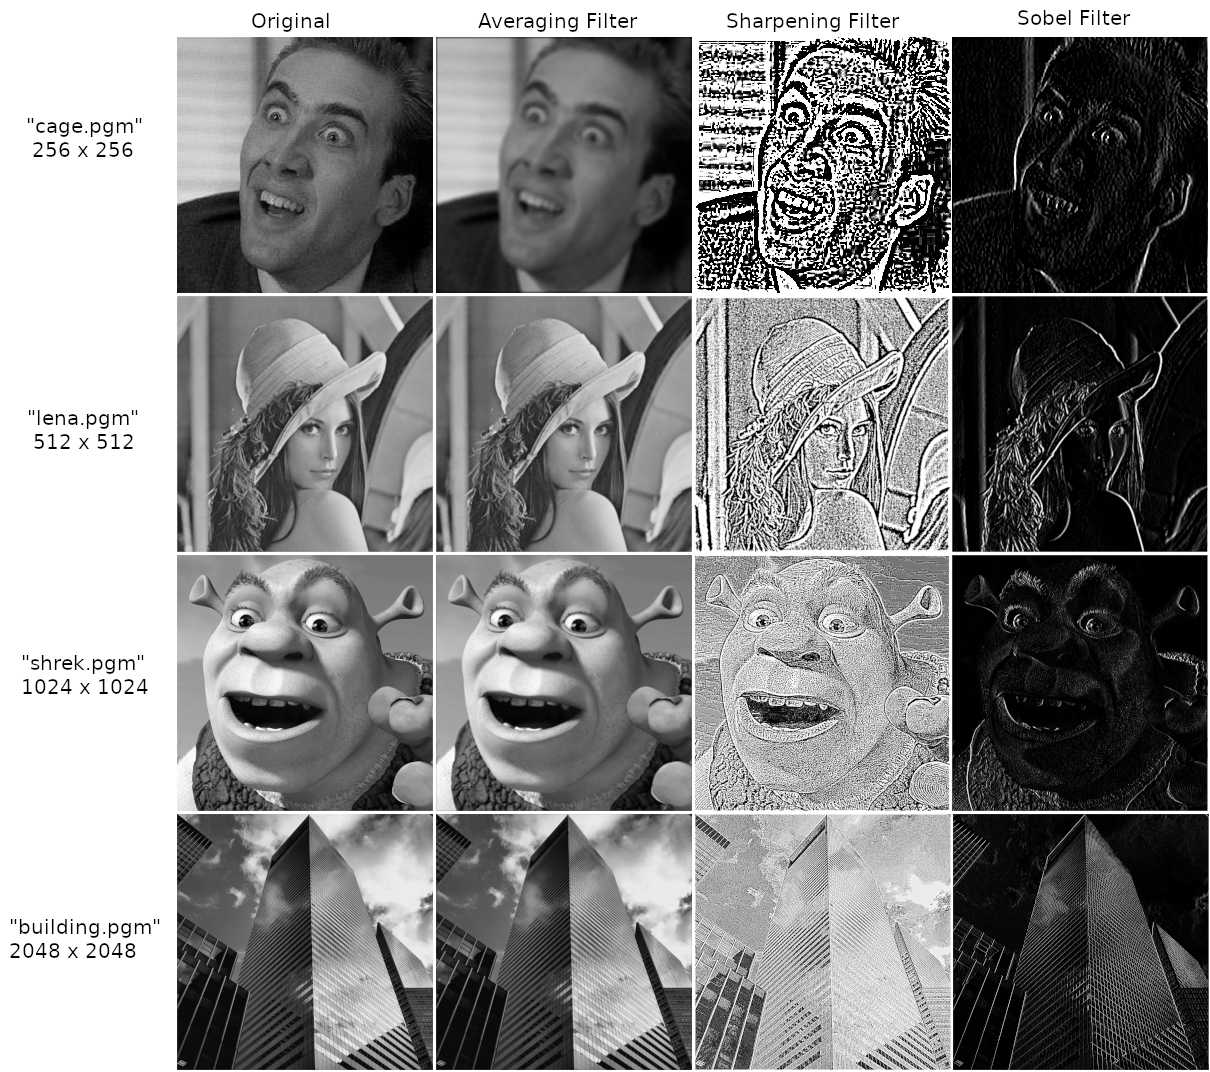
\includegraphics[scale=1.2]{images.png}
\end{figure}
\subsection{Kernel Time and Speedup}
This first set of results shows the execution time for the kernel for various image sizes and filter sizes using both the averaging and the sharpening filters. All times are in seconds.
\begin{table}[H]
\small
\begin{tabular}{ccccccc}
\multicolumn{7}{c}{\textbf{Averaging Filter - Kernel Time}}                                                                                                                                   \\
\textbf{Image Size}          & \textbf{Filter Size} & \textbf{Serial Time} & \textbf{Naive Time} & \textbf{Shared Memory Time} & \textbf{Constant Memory Time} & \textbf{Texture Memory Time} \\ \hline
\multirow{3}{*}{256 x 256}   & 3 x 3                & 0.014537             & 0.000041            & 0.000053                    & 0.000029                      & 0.00004                      \\
                             & 5 x 5                & 0.03184              & 0.000086            & 0.000103                    & 0.00005                       & 0.000062                     \\
                             & 9 x 9                & 0.058421             & 0.000208            & 0.000266                    & 0.000133                      & 0.000135                     \\ \hline
\multirow{3}{*}{512 x 512}   & 3 x 3                & 0.033477             & 0.000117            & 0.00016                     & 0.000076                      & 0.00009                      \\
                             & 5 x 5                & 0.047504             & 0.000293            & 0.000366                    & 0.000156                      & 0.000182                     \\
                             & 9 x 9                & 0.119374             & 0.000778            & 0.001178                    & 0.000415                      & 0.000488                     \\ \hline
\multirow{3}{*}{1024 x 1024} & 3 x 3                & 0.058487             & 0.000433            & 0.000592                    & 0.000268                      & 0.000301                     \\
                             & 5 x 5                & 0.12551              & 0.001128            & 0.001415                    & 0.000651                      & 0.00065                      \\
                             & 9 x 9                & 0.365407             & 0.003277            & 0.004373                    & 0.001771                      & 0.001693                     \\ \hline
\multirow{3}{*}{2048 x 2048} & 3 x 3                & 0.171482             & 0.001637            & 0.002689                    & 0.001026                      & 0.001283                     \\
                             & 5 x 5                & 0.442127             & 0.004866            & 0.00601                     & 0.002485                      & 0.002896                     \\
                             & 9 x 9                & 1.402518             & 0.012336            & 0.017509                    & 0.007144                      & 0.006652                    
\end{tabular}
\end{table}
\begin{table}[H]
\small
\begin{tabular}{ccccccc}
\multicolumn{7}{c}{\textbf{Sharpening Filter - Kernel Time}}                                                                                                                                                \\
\textbf{Image Size}          & \textbf{Filter Size} & \textbf{Serial Time} & \textbf{Naive Time} & \textbf{Shared Memory Time} & \textbf{Constant Memory Time} & \textbf{Texture Memory Time} \\ \hline
\multirow{3}{*}{256 x 256}   & 3 x 3                & 0.006454             & 0.000041            & 0.000052                    & 0.000029                      & 0.00004                      \\
                             & 5 x 5                & 0.010588             & 0.000086            & 0.000102                    & 0.000051                      & 0.000062                     \\
                             & 9 x 9                & 0.02632              & 0.000207            & 0.000281                    & 0.000115                      & 0.000132                     \\ \hline
\multirow{3}{*}{512 x 512}   & 3 x 3                & 0.01153              & 0.000118            & 0.000162                    & 0.000076                      & 0.000092                     \\
                             & 5 x 5                & 0.028605             & 0.000294            & 0.000363                    & 0.000155                      & 0.000179                     \\
                             & 9 x 9                & 0.086674             & 0.000792            & 0.001                       & 0.000416                      & 0.00045                      \\ \hline
\multirow{3}{*}{1024 x 1024} & 3 x 3                & 0.061758             & 0.000419            & 0.000591                    & 0.000267                      & 0.000295                     \\
                             & 5 x 5                & 0.112552             & 0.001127            & 0.001417                    & 0.000632                      & 0.000654                     \\
                             & 9 x 9                & 0.349421             & 0.003057            & 0.00395                     & 0.001751                      & 0.001675                     \\ \hline
\multirow{3}{*}{2048 x 2048} & 3 x 3                & 0.173789             & 0.001638            & 0.002322                    & 0.001027                      & 0.00111                      \\
                             & 5 x 5                & 0.452518             & 0.00447             & 0.005788                    & 0.002485                      & 0.002555                     \\
                             & 9 x 9                & 1.403984             & 0.012163            & 0.015792                    & 0.006965                      & 0.00662                     
\end{tabular}
\end{table}
We can immediately see that the time taken for the kernel function to run increases both with $M$ and $N$ but also with $L$ and $P$ as they increase for all approaches. This is of course predicted by the complexity analysis of these approaches.
\\
Restricting our discussion to the results of the sharpening filter, we can measure the speed-up, $S = \frac{Time_{Serial}}{Time_{Parallel}}$, of the various approaches and tabulate the results below:
\begin{table}[H]
\small
\begin{tabular}{cccccc}
\multicolumn{6}{c}{\textbf{Sharpening Filter - Speedup}}                                                                                                                        \\
\textbf{Image Size}          & \textbf{Filter Size} & \textbf{Naive Speedup} & \textbf{Shared Memory Speedup} & \textbf{Constant Memory Speedup} & \textbf{Texture Memory Speedup} \\ \hline
\multirow{3}{*}{256 x 256}   & 3 x 3                & 157.4146               & 124.1154                       & 222.5517                         & 161.3500                        \\
                             & 5 x 5                & 123.1163               & 103.8039                       & 207.6078                         & 170.7742                        \\
                             & 9 x 9                & 127.1498               & 93.6655                        & 228.8696                         & 199.3939                        \\ \hline
\multirow{3}{*}{512 x 512}   & 3 x 3                & 97.7119                & 71.1728                        & 151.7105                         & 125.3261                        \\
                             & 5 x 5                & 97.2959                & 78.8017                        & 184.5484                         & 159.8045                        \\
                             & 9 x 9                & 109.4369               & 86.6740                        & 208.3510                         & 192.6089                        \\ \hline
\multirow{3}{*}{1024 x 1024} & 3 x 3                & 147.3938               & 104.4975                       & 231.3034                         & 209.3492                        \\
                             & 5 x 5                & 99.8687                & 79.4298                        & 178.0886                         & 172.0979                        \\
                             & 9 x 9                & 114.3019               & 88.4610                        & 199.5551                         & 208.6096                        \\ \hline
\multirow{3}{*}{2048 x 2048} & 3 x 3                & 106.0983               & 74.8445                        & 169.2201                         & 156.5667                        \\
                             & 5 x 5                & 101.2345               & 78.1821                        & 182.0998                         & 177.1108                        \\
                             & 9 x 9                & 115.4307               & 88.9048                        & 201.5770                         & 212.0822                       
\end{tabular}
\end{table}
Here we see that the approach that consistently gives the highest speedup is the Constant Memory approach, followed by the Texture Memory approach, then the Na\"{i}ve approach and finally the Shared Memory approach. The fact that the Constant Memory approach is fastest is unsurprising, as it makes use of some of the fastest memory on the device. An interesting result is that the Shared Memory approach is the slowest. This is likely due to the increased overhead within the kernel required to handle the initialisation of the overlapping block.
\subsection{Global Memory Accesses}
Measuring the number of global memory accesses (read and write) performed by each approach, we arrive at the following results.
% Please add the following required packages to your document preamble:
% \usepackage{multirow}
\begin{table}[H]
\small
\begin{tabular}{cccccc}
\multicolumn{6}{c}{\textbf{Sharpening Filter - Global Memory Accesses}}                                                                            \\
\textbf{Image Size}          & \textbf{Filter Size} & \textbf{Naive} & \textbf{Shared Memory} & \textbf{Constant Memory} & \textbf{Texture Memory} \\ \hline
\multirow{3}{*}{256 x 256}   & 3 x 3                & 1245184        & 148480                 & 655360                   & 655360                  \\
                             & 5 x 5                & 3342336        & 167936                 & 1703936                  & 1703936                 \\
                             & 9 x 9                & 10682368       & 212992                 & 5373952                  & 5373952                 \\ \hline
\multirow{3}{*}{512 x 512}   & 3 x 3                & 4980736        & 593920                 & 2621440                  & 2621440                 \\
                             & 5 x 5                & 13369344       & 671744                 & 6815744                  & 6815744                 \\
                             & 9 x 9                & 42729472       & 851968                 & 21495808                 & 21495808                \\ \hline
\multirow{3}{*}{1024 x 1024} & 3 x 3                & 19922944       & 2375680                & 10485760                 & 10485760                \\
                             & 5 x 5                & 53477376       & 2686976                & 27262976                 & 27262976                \\
                             & 9 x 9                & 170917888      & 3407872                & 85983232                 & 85983232                \\ \hline
\multirow{3}{*}{2048 x 2048} & 3 x 3                & 79691776       & 9502720                & 41943040                 & 41943040                \\
                             & 5 x 5                & 213909504      & 10747904               & 109051904                & 109051904               \\
                             & 9 x 9                & 683671552      & 13631488               & 343932928                & 343932928              
\end{tabular}
\end{table}
As predicted by the results in Section \ref{ParallelApproaches}, we see that the number of global memory accesses in the Na\"{i}ve approach is equal to twice that of the Constant and Texture Memory approaches, and that the number corresponding to the Shared Memory approach is further scaled by the size of the tile. The fact that the number of global memory accesses does not correspond to the kernel execution time points to the effects of the various memory speeds and the overhead associated with each approach.
\subsection{Overhead Time}
The overhead time (that is, the time taken for the relevant variables to be initalised and copied from the host to the device and vice-versa) was measured for all approaches using both filter types. The following results were recorded.
\begin{table}[H]
\small
\begin{tabular}{cccccc}
\multicolumn{6}{c}{\textbf{Averaging Filter - Overhead Time}}                                                                                      \\
\textbf{Image Size}          & \textbf{Filter Size} & \textbf{Naive} & \textbf{Shared Memory} & \textbf{Constant Memory} & \textbf{Texture Memory} \\ \hline
\multirow{3}{*}{256 x 256}   & 3 x 3                & 0.084529       & 0.053155               & 0.0515                   & 0.051605                \\
                             & 5 x 5                & 0.082068       & 0.053767               & 0.053193                 & 0.052054                \\
                             & 9 x 9                & 0.073769       & 0.054243               & 0.054473                 & 0.057575                \\ \hline
\multirow{3}{*}{512 x 512}   & 3 x 3                & 0.074273       & 0.051962               & 0.052071                 & 0.053216                \\
                             & 5 x 5                & 0.074455       & 0.054641               & 0.054124                 & 0.054191                \\
                             & 9 x 9                & 0.071953       & 0.054384               & 0.05358                  & 0.056806                \\ \hline
\multirow{3}{*}{1024 x 1024} & 3 x 3                & 0.075182       & 0.053532               & 0.05368                  & 0.060639                \\
                             & 5 x 5                & 0.075999       & 0.0546                 & 0.055844                 & 0.05837                 \\
                             & 9 x 9                & 0.07342        & 0.054135               & 0.053048                 & 0.052906                \\ \hline
\multirow{3}{*}{2048 x 2048} & 3 x 3                & 0.080347       & 0.059241               & 0.054023                 & 0.054079                \\
                             & 5 x 5                & 0.076506       & 0.058069               & 0.055145                 & 0.055384                \\
                             & 9 x 9                & 0.089209       & 0.059943               & 0.054062                 & 0.057342               
\end{tabular}
\end{table}
\newpage
\begin{table}[H]
\small
\begin{tabular}{cccccc}
\multicolumn{6}{c}{\textbf{Sharpening Filter - Overhead Time}}                                                                                     \\
\textbf{Image Size}          & \textbf{Filter Size} & \textbf{Naive} & \textbf{Shared Memory} & \textbf{Constant Memory} & \textbf{Texture Memory} \\ \hline
\multirow{3}{*}{256 x 256}   & 3 x 3                & 0.066851       & 0.053856               & 0.05086                  & 0.051455                \\
                             & 5 x 5                & 0.060539       & 0.053923               & 0.052218                 & 0.052853                \\
                             & 9 x 9                & 0.063107       & 0.054783               & 0.055964                 & 0.052518                \\ \hline
\multirow{3}{*}{512 x 512}   & 3 x 3                & 0.063249       & 0.054889               & 0.052294                 & 0.053067                \\
                             & 5 x 5                & 0.066288       & 0.05473                & 0.051798                 & 0.050577                \\
                             & 9 x 9                & 0.064031       & 0.052632               & 0.051961                 & 0.051078                \\ \hline
\multirow{3}{*}{1024 x 1024} & 3 x 3                & 0.0644         & 0.053654               & 0.05364                  & 0.053326                \\
                             & 5 x 5                & 0.064512       & 0.053681               & 0.053515                 & 0.053266                \\
                             & 9 x 9                & 0.070299       & 0.053248               & 0.051807                 & 0.051805                \\ \hline
\multirow{3}{*}{2048 x 2048} & 3 x 3                & 0.069807       & 0.058458               & 0.055704                 & 0.056625                \\
                             & 5 x 5                & 0.070972       & 0.059943               & 0.055607                 & 0.063975                \\
                             & 9 x 9                & 0.065598       & 0.059443               & 0.062524                 & 0.055691               
\end{tabular}
\end{table}
We can immediately see that the overhead of the Na\"{i}ve approach is, as expected, substantially larger than that of the other approaches. On average, the Texture Memory approach has the least overhead, indicating that loading an image into texture memory may be more optimal than loading to the global memory. While the overhead time does increase with increases in $M$, $N$, $L$ and $P$, it does so minimally, with changes in time occurring in the order of 0.01 seconds, indicating that the connection between device and host is not much of a bottleneck in this problem and on this hardware.
\subsection{Measured Floating-point Computation Rate}
The floating-point computation rate, $FLOPS = \frac{f}{Time}$, where $f$ is the number of floating-point operations performed by the kernel, was calculated for each image size and filter size for each approach. The results are tabulated below, with all values in GFLOPS.
\begin{table}[H]
\small
\begin{tabular}{ccccccc}
\multicolumn{7}{c}{\textbf{Averaging Filter - FLOPS}}                                                                                                                \\
\textbf{Image Size}          & \textbf{Filter Size} & \textbf{Serial} & \textbf{Naive} & \textbf{Shared Memory} & \textbf{Constant Memory} & \textbf{Texture Memory} \\ \hline
\multirow{3}{*}{256 x 256}   & 3 x 3                & 0.41476         & 155.04859      & 780.24936              & 259.88414                & 158.92480               \\
                             & 5 x 5                & 0.51869         & 195.84595      & 503.29103              & 402.39104                & 271.65729               \\
                             & 9 x 9                & 0.91089         & 257.41785      & 332.85389              & 482.40409                & 396.61416               \\ \hline
\multirow{3}{*}{512 x 512}   & 3 x 3                & 0.72041         & 217.33306      & 1,033.83040            & 396.66526                & 282.53298               \\
                             & 5 x 5                & 1.39063         & 229.93518      & 566.54619              & 515.88595                & 370.17037               \\
                             & 9 x 9                & 1.78314         & 275.28489      & 300.64223              & 618.40717                & 438.87633               \\ \hline
\multirow{3}{*}{1024 x 1024} & 3 x 3                & 1.64941         & 234.90040      & 1,117.65449            & 449.94866                & 337.91320               \\
                             & 5 x 5                & 2.10534         & 238.90428      & 586.16510              & 494.48976                & 414.59082               \\
                             & 9 x 9                & 2.33012         & 261.42404      & 323.94836              & 579.64760                & 506.01689               \\ \hline
\multirow{3}{*}{2048 x 2048} & 3 x 3                & 2.25024         & 248.53237      & 984.23422              & 470.12179                & 317.10638               \\
                             & 5 x 5                & 2.39064         & 221.52407      & 552.02903              & 518.16955                & 372.21551               \\
                             & 9 x 9                & 2.42833         & 277.78424      & 323.63383              & 574.77934                & 515.14527              
\end{tabular}
\end{table}
\begin{table}[H]
\small
\begin{tabular}{ccccccc}
\multicolumn{7}{c}{\textbf{Sharpening Filter - FLOPS}}                                                                                                               \\
\textbf{Image Size}          & \textbf{Filter Size} & \textbf{Serial} & \textbf{Naive} & \textbf{Shared Memory} & \textbf{Constant Memory} & \textbf{Texture Memory} \\ \hline
\multirow{3}{*}{256 x 256}   & 3 x 3                & 0.93420         & 155.04859      & 795.25415              & 259.88414                & 158.92480               \\
                             & 5 x 5                & 1.55979         & 195.84595      & 508.22525              & 394.50102                & 271.65729               \\
                             & 9 x 9                & 2.02186         & 258.66141      & 315.08589              & 557.91082                & 405.62812               \\ \hline
\multirow{3}{*}{512 x 512}   & 3 x 3                & 2.09170         & 215.49125      & 1,021.06706            & 396.66526                & 276.39096               \\
                             & 5 x 5                & 2.30940         & 229.15309      & 571.22839              & 519.21425                & 376.37435               \\
                             & 9 x 9                & 2.45588         & 270.41875      & 354.15654              & 616.92062                & 475.93700               \\ \hline
\multirow{3}{*}{1024 x 1024} & 3 x 3                & 1.56205         & 242.74910      & 1,119.54561            & 451.63386                & 344.78601               \\
                             & 5 x 5                & 2.34773         & 239.11627      & 585.33777              & 509.35575                & 412.05509               \\
                             & 9 x 9                & 2.43673         & 280.23768      & 358.63954              & 586.26836                & 511.45468               \\ \hline
\multirow{3}{*}{2048 x 2048} & 3 x 3                & 2.22037         & 248.38064      & 1,139.79579            & 469.66403                & 366.52927               \\
                             & 5 x 5                & 2.33574         & 241.14902      & 573.20222              & 518.16955                & 421.89281               \\
                             & 9 x 9                & 2.42579         & 281.73529      & 358.82122              & 589.55113                & 517.63540              
\end{tabular}
\end{table}
Here the strengths of GPU parallelisation are evident, with FLOPS scaling vastly compared to the serial approach. As expected, the Na\"{i}ve approach has a low floating-point computation rate when compared to the other approaches, although it is still substantially higher than the serial approach. We see the highest FLOPS in the Shared Memory approach, likely because the internal overhead is still large despite relatively few floating-point operations. Even then, the performance here is only a fraction of the theoretical maximum.
\\
The general trend is that FLOPS increases with increases in $M$, $N$, $L$ and $P$. This is true for all approaches except the Shared Memory approach, whose FLOPS increases with increasing $M$ and $N$ but actually decreases with higher values of $L$ and $P$. This is because the kernel time grows faster than the number of operations, as a smaller proportion of floating-point operations are dependent on $L$ and $P$ than in other kernels.
\section{Conclusion}
We conclude that the image convolution problem is a prime example of algorithms whose performances can be improved substantially by parallel approaches. After running the tests detailed in Section \ref{EmpiricalAnalysis}, we note that the best performance is achieved by the Constant Memory approach, and then by the Texture Memory approach. We hypothesize that the ideal parallel convolution algorithm would be a hybrid solution in which the image is loaded into texture memory while the filter is loaded into constant memory, as this approach maximises memory access speed while keeping overhead costs reasonable. Further work could include implementation of this approach, as well as other optimisation such as making use of the separability of certain filters.
\bibliographystyle{IEEEannot}
\bibliography{myBib}

\end{document} 

